% !TEX root = BA-Bauer

\subsection{Schaltungsprinzip}

In diesem Kapitel wird auf das grundlegende Prinzip der Schlatung eingegangen. Auf die einzelnen Komponenten und deren nötige Beschaltung wird in den folgenden Kapiteln eingegangen. Generell wird bei der Entwicklung der Schaltung darauf geachtet, dass möglichst keine fertigen Modulbausteine verwendet werden. Dadurch ergibt sich in der Regel ein Preisvorteil und das industrielle Bestücken einer Platine ist einfacher.%(Quelle?)
Abbildung \ref{fig:Schaltungsrinzip} zeigt das grundlegende Prinzip der Schaltung. Auf der linken Seite steht der Benutzer des Gerätes, der das Gerät durch Eingaben bedienen kann und entsprechende Rückmeldungen erhält. Die grüne Fläche spiegelt dasGerät wieder, welches mit der DMX-Quelle, bzw. der DMX-fähigen Lichttechnik kommuniziert. Im Folgenden wird auf die Bestandteile des Gerätes eingegangen.

\vspace*{5mm}
\begin{figure}[h]
	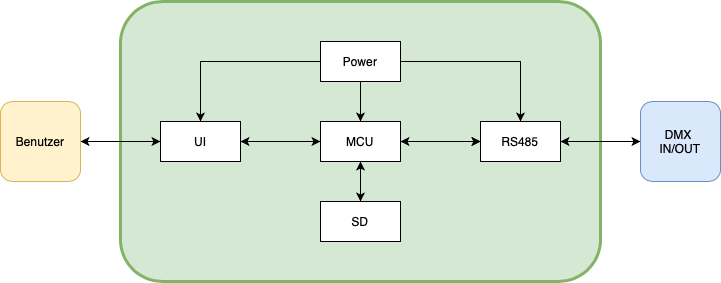
\includegraphics[width = \textwidth]{Schaltungsprinzip}
	\caption{Schaltungsprinzip}
	\label{fig:Schaltungsrinzip}
\end{figure}
\hspace*{-5mm}\textbf{Mikrocontroller (MCU)}\\
Der MCU bildet das Herzstück der Schaltung, über den sämtliche Kommunikation für die Benutzerschnittstelle, den DMX-Ein- und Ausgang und die SD-Karte läuft. Aufrgund der hohen Anforderungen an den MCU wird bei der Entwicklung ein besonderes Augenmerk auf ihn gelegt. Die Auswahl des MCUs richtet sich an dem in der vorangegangen Praxisprojektarbeit verwendeten Mikrocontroller. Auswahlkriterien sind eine mindestens gleichhohe Taktfrequenz des Prozessors, eine verfügbare UART-Schnittstelle, eine SDIO-Schnittstelle und mindestens drei Timer.\\
\textbf{Spannungsversorgung (Power)}\\
Die Spannungsversorgung für alle Komponenten wird von einer USB Schnittstelle geliefert, welche keine Daten übertragt. Über die USB-Schnittstelle werden 5V geliefert (Quelle), welche dann in enstprechend benötigte Spannungen gewandelt werden. Besonders kritisch ist die Versorgung des MCUs. Unter normalen Betriebsbedingungen darf die Versorgungsspannung nur soweit einbrechen, dass der MCU weiterhin den darauf befindlichen Programmcode fehlerfrei ausführen kann.\\
\textbf{Benutzerschnittstelle (UI)}\\
Damit der Benutzer das Gerät bedienen kann, ist ein Informationsfluss in zwei Richtungen eforderlich. Zum einen müssen Eingaben durch den Benutzer erfasst werden, zum anderen muss das Gerät dem Benutzer eine Rückmeldung ausgeben können. Für die Benutzereingaben werden Taster und ein Drehgeber (Encoder) verwendet. Durch den Einsatz von Tastern können präzise und zeitgenaue Eingaben vom Benuter vorgenommen werden, an Stellen an denen es nötig ist, zum Beispiel beim starten einer Wiedergabe. Der Encoder hingegen bietet die Möglichkeit viele Eingaben in kurzer Zeit zu tätigen, zum Beispiel wenn die Aufnahmezeit eingestellt wird.\\
\textbf{RS485}\\
Die RS485-Schnittstelle ist die Verbindung zwischen DMX-Quelle/Senke und dem MCU, welche notwendig ist, da der MCU keine RS485 konformen Signalpegel liefern kann. Zudem werden durch die Schnittstelle die DMX-Leitungen galvanisch von der restlichen Schaltung getrennt. Spannungs- und Stromspitzen ausgehend von den DMX-Leitungen können so die Schaltung nicht beeinträchtigen oder beschädigen.\\
\textbf{Speicher (SD-Karte)}\\
Damit ein sinnvoler Einsatz des Gerätes mögilch ist, ist es notwendig die aufgenommenen Daten auf einem Speichermedium zu sichern und diese nach einen Neustart des Gerätes nach wie vor verfügbar sind. In der vorangegangen Praxisprojektabreit wurde bereits gezeigt, dass der Einsatz einer SD-Karte für diesen Zweck geeignet ist. Die Verwendung einer SD-Karte ermöglicht dem Benutzer außerdem eine gewisse Sicherheit in Bezug auf den Schutz der Daten. Sollte ein Gerät einen Defekt aufweisen, so kann einfach ein neues Gerät mit der bereits beschriebenen SD-Karte bestückt werden. Zudem können für verschiedene Einsatzgbiete auch verschiede SD-Karten verwendet werden.